\section{System Design}
\label{sec:design}
The runtime exposes named operations through two entry paths. In a task, a registered harness gives the agent scoped tools to read process data and submit a proposed change. External callers can invoke the same tools through the Representational State Transfer (REST) interface or the standard-I/O MCP bridge. Both paths enter the shared dispatcher. Scene configuration supplies the production context and the mappings and limits the handlers use.

\begin{figure*}[!t]
\centering
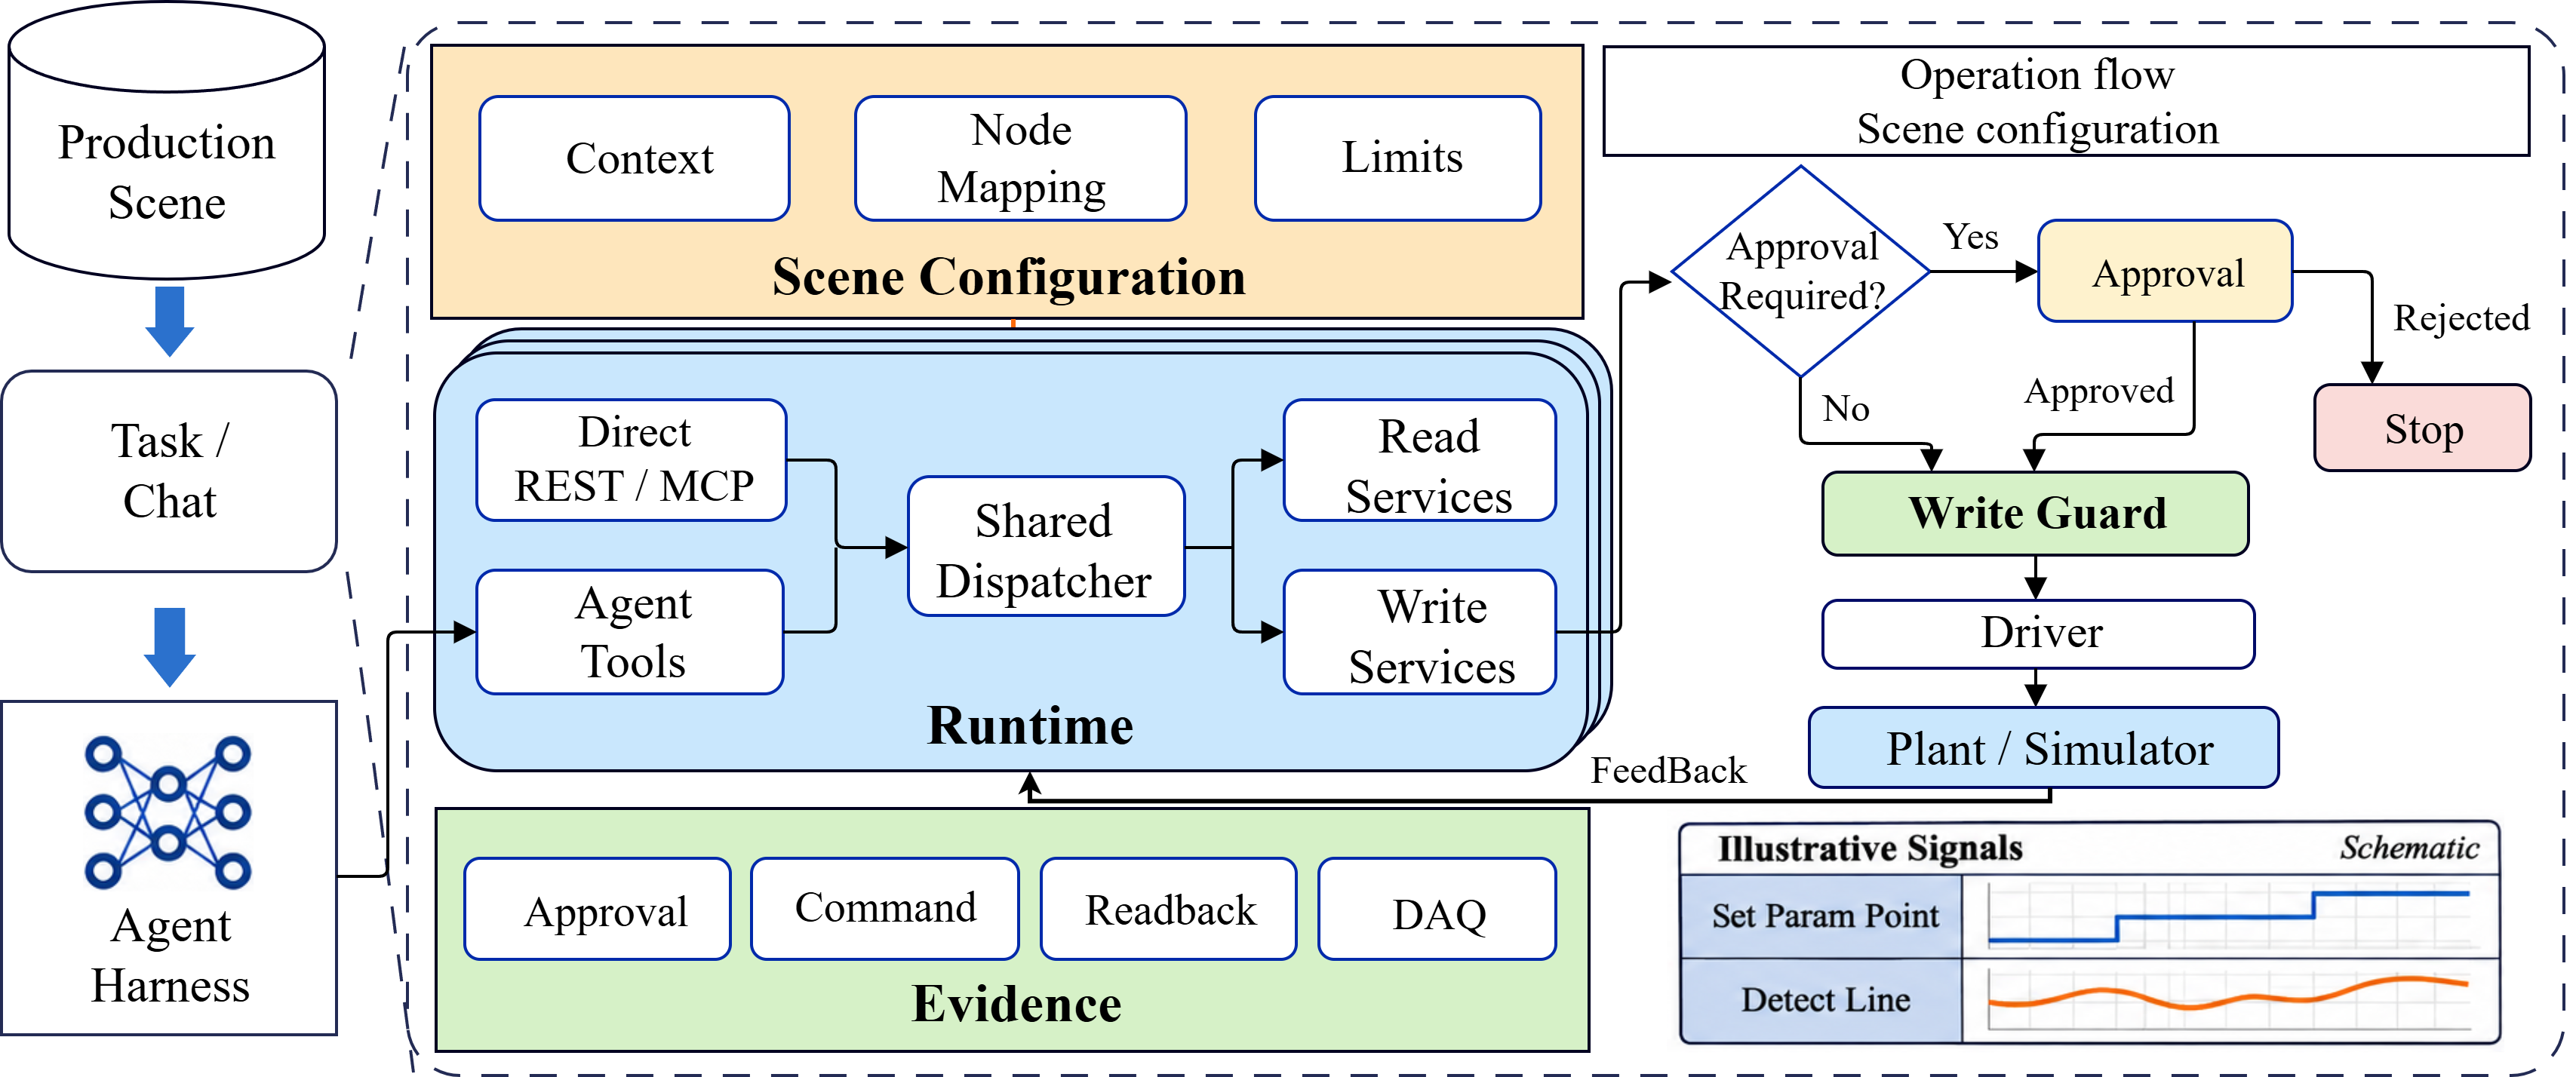
\includegraphics[width=\textwidth]{resources/fig2.png}
\caption{Scene configuration, shared dispatch, and governed write execution. Task-mediated and direct tool calls reach the same dispatcher. Every write follows the applicable authorization and guard checks. A required approval triggers route-specific revalidation (Fig.~\ref{fig:hitl}). Only an admitted command reaches the driver. Approval, command outcome, optional readback, and subsequent data acquisition (DAQ) produce separate records. The inset illustrates setpoint and process signals schematically.}
\label{fig:arch}
\end{figure*}

\subsection{Design Rationale and Requirements}
\label{sec:principles}
The agent uses production context and available observations to decide what to propose. The operation handler determines whether it can execute that proposal against the current state. Keeping those decisions separate lets the harness present the same tools across scenes while the runtime checks the applicable node bindings, authority, and limits for each write.

\subsection{Layered Architecture}
\label{sec:layers}
Fig.~\ref{fig:arch} shows how task and chat calls enter the runtime through a harness, while direct tool calls reach the dispatcher without a task. The dispatcher routes reads to DAQ, MES access, retrieval, or other analysis services and writes to node or recipe services. The services use configured input and output mappings to reach built-in or plugin drivers. The administrative node-write interface used in Section~\ref{sec:eval-mapping} exercises the downstream write controller independently of task and agent-tool dispatch.

\subsection{Scene Configuration as the Integration Boundary}
\label{sec:scene-config}
The active line identifies the production context. Product and recipe records supply targets and limits, and the run record supplies the operating state. Each semantic node names a process variable and specifies its direction, unit, and mapping. The registry resolves that mapping to a registered driver. The harness calls a named, typed operation without constructing a protocol message. A new scene can bind existing drivers through configuration. Adding support for another protocol requires a driver adapter.

In the cast-film simulator preset, for example, the MQTT command mapping
\texttt{linespeed-sp} controls line speed in m/min, while the distinct
\texttt{film-thickness} mapping supplies thickness in $\mu$m. An agent can
acquire the thickness observation, compare it with its objective, and propose a
line-speed adjustment. The runtime checks the proposal against the speed node's
limits and sends an admitted command to its MQTT mapping.

Table~\ref{tab:scene-config} shows where the runtime uses each configuration element. Before dispatch, the handler resolves the live state required by its route. Recipe operations bind approval to both the proposal and the active production context.

\begin{table*}[!t]
\centering
\caption{Scene configuration elements and their roles in the runtime path.}
\label{tab:scene-config}
\footnotesize
\setlength{\tabcolsep}{5pt}
\begin{tabularx}{\textwidth}{@{}>{\raggedright\arraybackslash}p{0.19\textwidth}>{\raggedright\arraybackslash}p{0.34\textwidth}X@{}}
\toprule
Element & Configured information & Runtime use\\
\midrule
Production context & Line, product, recipe, and run associations & Context construction for a task turn; route-dependent live-state checks before a write\\
Semantic I/O & Process variable, direction, unit, and node mapping & Acquisition uses the read mapping; accepted operations resolve the configured control mapping\\
Driver binding & Supported protocol driver and endpoint configuration & Driver registry selects the protocol implementation after operation checks\\
Operation admission & Engineering, baseline, product, and recipe limits; step and timing rules where configured & Route handler checks the candidate against current bounds and rejects inadmissible requests\\
Approval policy & Whether approval is required and the decision validity window & Pending request binds the proposed action; route-specific checks run after approval\\
Evidence ownership & Command receipt, verification grade, and later DAQ observations & Owning services retain command outcomes separately from process measurements\\
\bottomrule
\end{tabularx}
\end{table*}

\subsection{Cross-Module Execution Flow}
\label{sec:executionflow}
For a task-mediated call, the registered adapter presents a scoped tool
catalog containing acquisition, context, and control operations to the agent.
The agent reads available observations, relates them to the task objective, and
submits a typed intent rather than a protocol-specific message. At the
operation boundary, the shared dispatcher checks the predicates declared for
the named operation before selecting its handler. The handler resolves live
production state, applies route-specific guards and limits, and requests any
required approval before device I/O.

For an industrial operation $u$ by agent $a$ in channel $c$, define the
shared dispatch condition as
\begin{equation}
\mathcal{A}(a,c,u)=\bigwedge_{X\in\mathcal{C}(u)}X(a,c,u).
\label{eq:dispatch-contract}
\end{equation}
In Eq.~(\ref{eq:dispatch-contract}), $S$, $P$, $G$, and $B$ denote invocation scope, current channel policy,
applicable industrial grant, and the agent's binding to referenced resources,
respectively. $\mathcal{C}(u)\subseteq\{S,P,G,B\}$ is the set of predicates
declared for operation $u$; it always contains $S$ and $P$. The grant predicate
$G$ is included when the resolved channel, target line, and owner/grant policy
require it; explicit exemptions omit it. The binding predicate $B$ is included
when the operation declares resource references. An operation that declares
no references omits $B$. Each included check must pass before handler
selection. The policy predicate includes channel tool selection, profile, and duty-separation checks where
configured.

Once these predicates pass, the selected route applies its operational
guards and requests any required approval. For example, an exploration request checks
the control binding and DAQ visibility before entering the governed write
path; an invisible target returns an error before a write. The checks performed
after approval depend on the route; Section~\ref{sec:modules} specifies the
single-node and recipe-operation paths.

For a direct REST agent-tool call, the service establishes $a$ and $c$ before applying
these checks. An agent token must match the requested agent identifier; an
authenticated user must be the channel owner or an administrator. The manager
loads the channel-agent record and rechecks scope and policy, followed by any
applicable grant and binding checks. Handlers resolve live production state
using request identifiers and the owning services.


